\documentclass[a4paper,landscape,columns=3,english]{cheatsheet}

\usepackage[utf8]{inputenc}
\usepackage[T1]{fontenc}
\usepackage[english]{babel}
\usepackage{tikz}
\usepackage{tikz-cd}
\usetikzlibrary{fit}
\usepackage{pgf-umlsd}
\usepackage{tcolorbox}
\usepgflibrary{arrows} % for pgf-umlsd
\usepackage{graphicx}
\usepackage{epstopdf}


\AfterPreamble{\hypersetup{
            pdfauthor={(C) Ilya Pronin, 2018},
            pdftitle={Python Multithreading and Multiprocessing Concepts in Diagrams},
            pdfsubject={Python},
            pdfkeywords={python multithreading multiprocessing process thread synchronization primitive}
}}
            

\author{(C) Ilya Pronin, 2018}

\title{Python Multithreading and Multiprocessing Concepts in Diagrams}

  
\begin{document}

  \newcommand{\labelmp}[0]{ \textsuperscript{ \tiny{ \colorbox{pink}{process} } } }
  \newcommand{\labelth}[0]{ \textsuperscript{ \tiny{ \colorbox{yellow}{thread} } } }
  \newcommand{\labelnomac}[0]{ \textsuperscript{ \tiny{ \colorbox{magenta}{no MacOS} } } }

  \section{Synchronization Primitives}

  \subsection{Lock \labelmp \labelth}
  
    \noindent
    \begin{tikzcd}[]     
      Thread \arrow[r, bend left=40,"acquire"{name=U, above, draw=red}]
        \arrow[r, bend right=40,"release"{name=D, below, draw=red}]
        & Lock         
    \end{tikzcd}
    
  \subsection{RLock \labelmp \labelth}
  
    \noindent
    \begin{tikzcd}[]         
      Thread \arrow[rd, bend left=40,"acquire"{name=U, above, draw=red}] \\
       & RLock \arrow[r] & { \begin{tabular}{l}
        \textbf{pid::}owner \\
        \textbf{int::}count
       \end{tabular} } \\    
      Thread \arrow[ru, bend right=40,"release"{name=D, below, draw=red}]
    \end{tikzcd}
    
  \subsection{Condition \labelmp \labelth}
  
    1 or more wait until notified
  
    \noindent
    \begin{tikzcd}[]
      Thread
      \arrow[rd, bend left=40, shift left=3,"release"{above, draw=red}]
      \arrow[rd, bend left=40, shift left=0,"notify"{right, draw=red}]
      \arrow[rd, bend left=40, shift right=3,"acquire"{below, draw=red}]
      \arrow[rd, bend left=0, shift left=0,"notify\_all"{below, draw=red}]
      \\
       & Condition \arrow[r] & { \begin{tabular}{l}
        \textbf{Lock::}lock \\
        \textbf{dequeue::}waiters \\
        \textbf{pid::}owner
       \end{tabular} } \\    
       Thread
       \arrow[ru, bend right=40, shift left=3,"acquire"{above, draw=red}]
       \arrow[ru, bend right=40, shift left=0,"wait"{right, draw=red}]
       \arrow[ru, bend right=40, shift right=3,"release"{below, draw=red}]
    \end{tikzcd}
    
  \subsection{Semaphore \labelmp \labelth}
  
    \noindent
    \begin{tikzcd}
      Thread \arrow[rd, bend left=40,"acquire"{name=U, above, draw=red}] \\
       & Semaphore \arrow[r] & { \begin{tabular}{l}
        \textbf{Condition::}condvar \\
        \textbf{int::}value
       \end{tabular} } \\    
      Thread \arrow[ru, bend right=40,"release"{name=D, below, draw=red}]
    \end{tikzcd}
    
  \subsection{BoundedSemaphore \labelmp \labelth \labelnomac}
  
  ValueError is raised if value $>$ initial
  
    \noindent
    \begin{tikzcd}
      Thread \arrow[rd, bend left=20,"acquire"{name=U, above, draw=red}] \\
       & BoundedSemaphore \arrow[r] & { \begin{tabular}{l}
        \textbf{Condition::}condvar \\
        \textbf{int::}initial \\
        \textbf{int::}value
       \end{tabular} } \\    
      Thread \arrow[ru, bend right=20,"release"{name=D, below, draw=red}]
    \end{tikzcd}
    
  \subsection{Event \labelmp \labelth}
  
    \noindent
    \begin{tikzcd}
      Thread \arrow[r, bend left=40,"set"{name=U, above, draw=red}]
             \arrow[r, bend left=20,"clear"{name=D, below, draw=red}]
             \arrow[r, bend right=20,"wait"{name=D, below, draw=red}]
             \arrow[r, bend right=40,"is\_set"{name=D, below, draw=red}]
       & Event \arrow[r] & { \begin{tabular}{l}
        \textbf{Condition::}condvar \\
        \textbf{bool::}flag
       \end{tabular} }
    \end{tikzcd}
    
  \subsection{Timer \labelth}
  
    \noindent
    \begin{tikzcd}
      Thread \arrow[r, bend left=20,"run"{name=U, above, draw=red}]
             \arrow[r, bend right=20,"cancel"{name=D, below, draw=red}]
       & Timer \arrow[r] & { \begin{tabular}{l}
        \textbf{Event::}finished \\
        \textbf{int::}interval \\
        \textbf{function::}f \\
        \textbf{list::}args \\
        \textbf{dict::}kwargs
       \end{tabular} }
    \end{tikzcd}
    
  \subsection{Barrier \labelmp \labelth}
  
    \noindent
    \begin{tikzcd}
      Thread
      \arrow[r, bend left=40,"wait"{name=U, above, draw=red}]
      \arrow[r, bend left=20,"reset"{name=U, above, draw=red}]
      \arrow[r, bend right=40,"abort"{name=U, above, draw=red}]
      & Barrier \arrow[r] & { \begin{tabular}{l}
        \textbf{Condition::}condvar \\
        \textbf{function::}action \\
        \textbf{int::}timeout \\
        \textbf{int::}parties \\
        \textbf{int::}n\_waiting \\
        \textbf{int::}count \\
        \textbf{int::}state $\in$ \{ Filling \\ Draining \\ Resetting \\ Broken \}
       \end{tabular} }
    \end{tikzcd}
  
  \subsection{Thread-Local Data \labelth}
  
    \noindent
    \begin{tikzcd}
      Thread
      \arrow[r, bend left=40,"getattr"{name=U, above, draw=red}]
      \arrow[r, bend left=0,"setattr"{name=U, above, draw=red}]
      \arrow[r, bend right=40,"setdefault"{name=U, above, draw=red}]
      & local \arrow[r] & { \begin{tabular}{l}
        \textbf{dict::}\_\_dict\_\_
       \end{tabular} }
    \end{tikzcd}
  
  \subsection{Exception}
  
  Convert an Exception instance to string before passing to the different thread
  
  \subsection{Signal}
  
  Signal can be caught inside any thread, but handling is only allowed within Main Thread
  
  \noindent
  \begin{tikzcd}
    Main Thread \arrow[rd,"receive"{below}] \arrow[r,"register"] & Handler Function \\
    & Signal \arrow[r] & Native Handler \arrow[lu,"deferred\ call"{above}]  \\
    Thread \arrow[ru,"receive"] \\
  \end{tikzcd}  
  
  
  \section{Inter-Process Communication}
  
  \subsection{Queue \labelmp}
  
    \noindent
    \begin{tikzcd}
      Thread
      \arrow[r, bend left=90,"get"{name=U, above, draw=red}]
      \arrow[r, bend left=50,"put"{name=U, above, draw=red}]
      \arrow[r, bend left=30,"qsize \labelnomac"{name=U, above, draw=red}]
      \arrow[r, bend left=20,"empty"{name=U, above, draw=red}]
      \arrow[r, bend right=0,"get\_nowait"{name=U, above, draw=red}]
      \arrow[r, bend right=30,"put\_nowait"{name=U, below, draw=red}]
      \arrow[r, bend right=50,"close"{name=U, below, draw=red}]
      \arrow[r, bend right=90,"join\_thread"{name=U, below, draw=red}]
      & SimpleQueue \arrow[r] & { \begin{tabular}{l}
        \textbf{Pipe::}pipe \\
        \textbf{int::}maxsize \\
        \textbf{Lock::}lock \\
        \textbf{pid::}owner \\
        \textbf{BoundedSemaphore::}sem
       \end{tabular} }
    \end{tikzcd}
    
  \subsection{Pipe \labelmp}
  
    \noindent
    \begin{tikzcd}
      Thread
      \arrow[r, bend left=90,"send"{name=U, above, draw=red}]
      \arrow[r, bend left=50,"recv"{name=U, above, draw=red}]
      \arrow[r, bend left=20,"close"{name=U, above, draw=red}]
      \arrow[r, bend right=50,"recv\_bytes"{name=U, below, draw=red}]
      \arrow[r, bend right=80,"send\_bytes"{name=U, below, draw=red}]
      & SimpleQueue \arrow[r] & { \begin{tabular}{l}
        \textbf{Connection::}conn1 \\
        \textbf{Connection::}conn2
       \end{tabular} }
    \end{tikzcd}
    
  \subsection{SimpleQueue}
    
    \noindent
    \begin{tikzcd}
      Thread
      \arrow[r, bend left=40,"get"{name=U, above, draw=red}]
      \arrow[r, bend left=0,"put"{name=U, above, draw=red}]
      \arrow[r, bend right=40,"empty"{name=U, above, draw=red}]
      & SimpleQueue \arrow[r] & { \begin{tabular}{l}
        \textbf{Pipe::}pipe \\
        \textbf{Lock::}lock
       \end{tabular} }
    \end{tikzcd}
  
  \subsection{JoinableQueue \labelmp}
  
    \noindent
    \begin{tikzcd}
      Thread
      \arrow[r, bend left=40,"get"{name=U, above, draw=red}]
      \arrow[r, bend left=20,"put"{name=U, above, draw=red}]
      \arrow[r, bend right=0,"empty"{name=U, above, draw=red}]
      \arrow[r, bend right=20,"task\_done"{name=U, above, draw=red}]
      \arrow[r, bend right=40,"join"{name=U, above, draw=red}]
      & JoinableQueue \arrow[r] & { \begin{tabular}{l}
        \textbf{Queue::}self \\
        \textbf{Semaphore::}unfinished\_tasks \\
        Condition::condvar 
       \end{tabular} }
    \end{tikzcd}
  
  \section{How Condition Works}
 
    \begin{sequencediagram}
    
      \newthread{p1}{p1}
      \newthread{p2}{p2}
      \newthread{cond}{Condition}
      \newthread{lock}{Lock}
      
      \begin{call}{p2}{acquire()}{cond}{}
        \begin{call}{cond}{acquire()}{lock}{}
        \end{call}
      \end{call}
      
      \begin{call}{p2}{wait()}{cond}{}
        
        \begin{call}{p1}{acquire()}{cond}{}
        \end{call}       
        
        \begin{call}{p1}{notify()}{cond}{}
        \end{call}       
        
        \begin{call}{p1}{release()}{cond}{}
        \end{call}       
        
        \begin{call}{cond}{acquire()}{lock}{}
        \end{call}       
      
    \end{call}
        
    \begin{call}{p2}{release()}{cond}{}
        \begin{call}{cond}{acquire()}{lock}{}
        \end{call}
    \end{call}       
    
  \end{sequencediagram}
  
  \section{Clusters and Pools}
  
  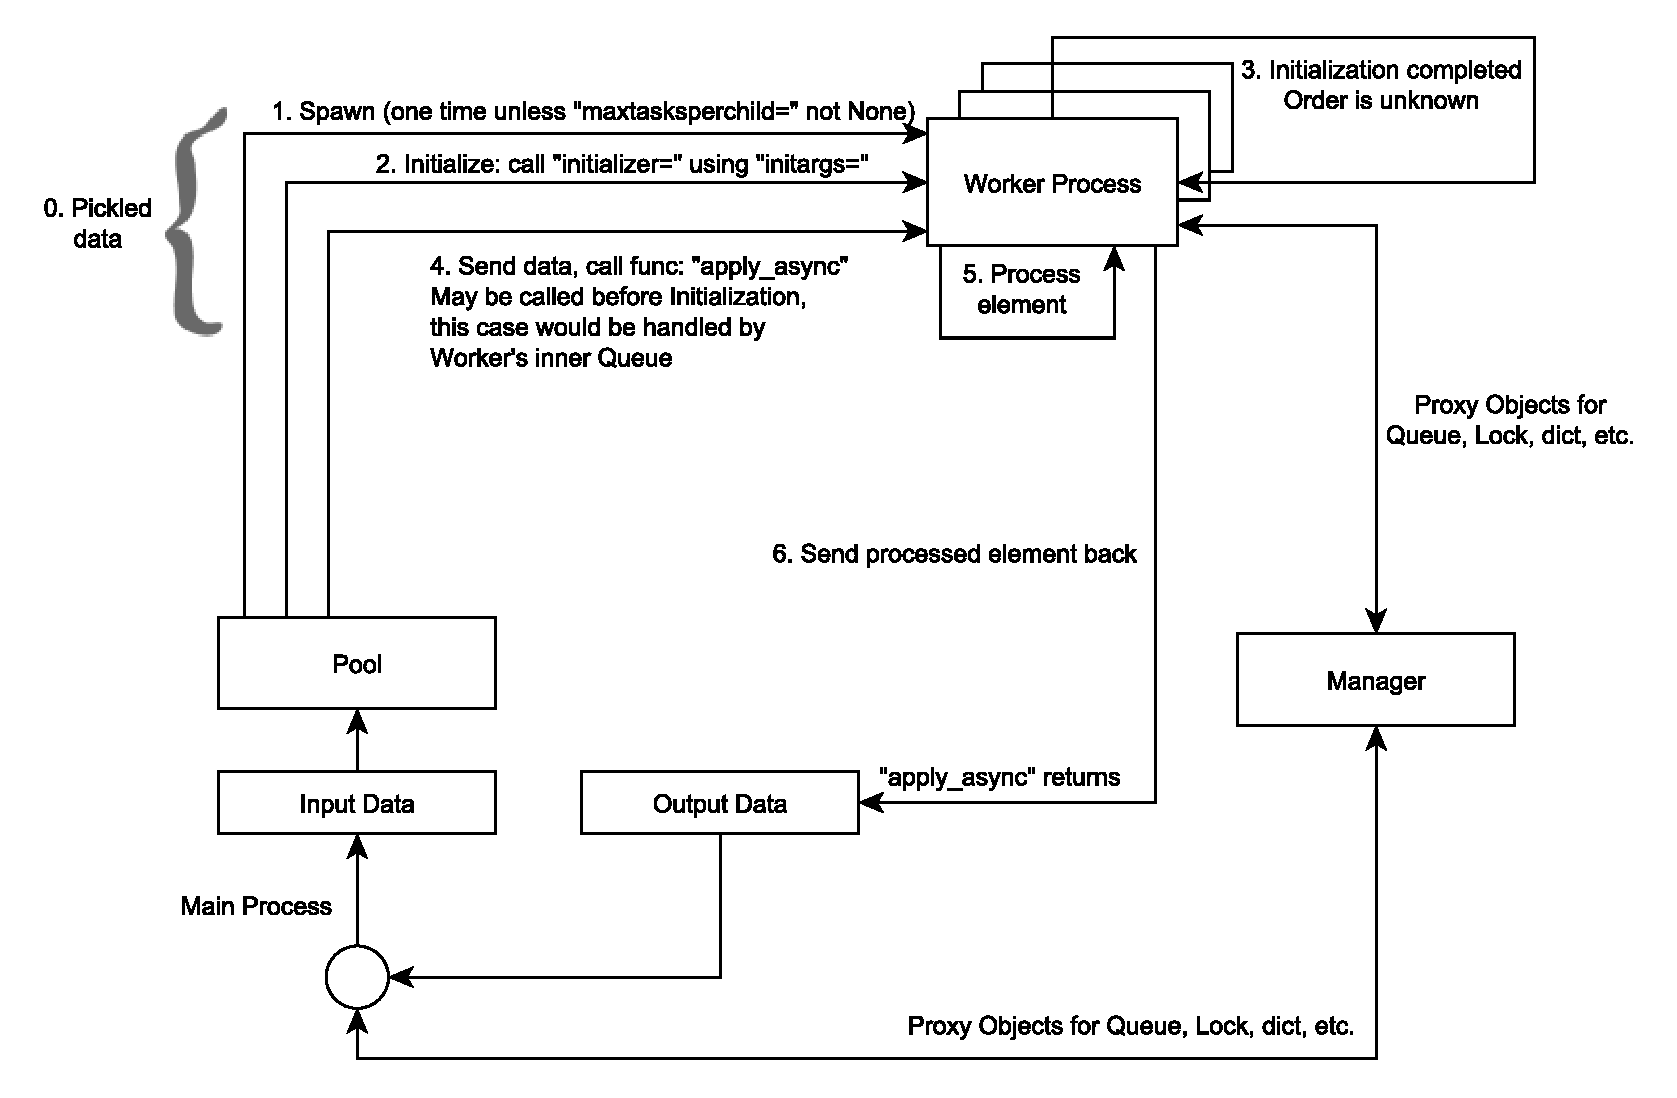
\includegraphics[trim = 0mm 0mm 0mm 0mm, clip, width=15cm]{apply_async}
  
\end{document}